\documentclass[11pt,a4paper]{report}

% -----------------------------------------------------------------------------
% PACKAGE IMPORTS & CONFIGURATION
% -----------------------------------------------------------------------------
\usepackage[utf8]{inputenc}
\usepackage[T1]{fontenc}
\usepackage{geometry}
\geometry{
    top=2.0cm,
    bottom=2.0cm,
    left=2.3cm,
    right=2.3cm,
    headheight=14.5pt
}

\usepackage{graphicx}
\usepackage{xcolor}
\usepackage{fancyhdr}
\usepackage{hyperref}
\usepackage{listings}
\usepackage{booktabs}
\usepackage{tabularx}
\usepackage{tikz}
\usetikzlibrary{shapes.geometric, arrows, positioning, fit, backgrounds, calc}
\usepackage{titlesec}
\usepackage{setspace}
\usepackage{amsmath,amssymb}
\usepackage{enumitem}

% Color Definitions
\definecolor{iiitblue}{RGB}{14, 43, 92}
\definecolor{dockerblue}{RGB}{13, 136, 230}
\definecolor{darknavy}{RGB}{11, 15, 25}
\definecolor{codegray}{RGB}{245, 247, 250}
\definecolor{codeborder}{RGB}{209, 213, 219}
\definecolor{codegreen}{RGB}{16, 149, 93}
\definecolor{codepurple}{RGB}{128, 0, 128}

% Hyperref Setup
\hypersetup{
    colorlinks=true,
    linkcolor=iiitblue,
    filecolor=dockerblue,
    urlcolor=dockerblue,
    citecolor=codegreen,
    pdftitle={CloudBox - Docker-Based Cloud Storage System},
    pdfauthor={Karthik Chakala, Shaik Venkat},
    pdfsubject={Docker and Containerization Project Report}
}

% YAML language definition for listings
\lstdefinelanguage{yaml}{
  keywords={true,false,null,y,n,services,networks,volumes,version,image,build,context,dockerfile,ports,environment,depends_on,restart,healthcheck,driver,command,deploy,resources,limits,cpus,memory},
  keywordstyle=\color{dockerblue}\bfseries,
  basicstyle=\ttfamily\scriptsize,
  sensitive=false,
  comment=[l]{\#},
  commentstyle=\color{codegreen}\itshape,
  stringstyle=\color{codepurple},
  moredelim=[l][\color{darknavy}]{\:},
  morestring=[b]',
  morestring=[b]"
}

% Code Listing Configuration
\lstdefinestyle{mystyle}{
    backgroundcolor=\color{codegray},
    commentstyle=\color{codegreen}\itshape,
    keywordstyle=\color{dockerblue}\bfseries,
    numberstyle=\tiny\color{gray},
    basicstyle=\ttfamily\scriptsize,
    breakatwhitespace=false,
    breaklines=true,
    captionpos=b,
    keepspaces=true,
    numbers=none,
    showspaces=false,
    showstringspaces=false,
    showtabs=false,
    tabsize=2,
    frame=single,
    rulecolor=\color{codeborder},
    xleftmargin=6pt,
    xrightmargin=6pt
}
\lstset{style=mystyle}

% Page Header and Footer Styling
\pagestyle{fancy}
\fancyhf{}
\fancyhead[L]{\small\textbf{CloudBox} --- Docker-Based Cloud Storage System}
\fancyhead[R]{\small IIITDM Kurnool}
\fancyfoot[L]{\small Department of Computer Science \& Engineering}
\fancyfoot[R]{\thepage}
\renewcommand{\headrulewidth}{0.6pt}
\renewcommand{\footrulewidth}{0.4pt}

% Title Format Customization
\titleformat{\chapter}[hang]{\normalfont\Large\bfseries\color{iiitblue}}{\thechapter.}{0.6em}{}
\titlespacing*{\chapter}{0pt}{-14pt}{8pt}
\titleformat{\section}{\normalfont\normalsize\bfseries\color{dockerblue}}{\thesection}{0.5em}{}
\titlespacing*{\section}{0pt}{6pt}{2pt}
\titleformat{\subsection}{\normalfont\small\bfseries\color{darknavy}}{\thesubsection}{0.4em}{}
\titlespacing*{\subsection}{0pt}{4pt}{1pt}

\setstretch{1.08}

% -----------------------------------------------------------------------------
% DOCUMENT BODY
% -----------------------------------------------------------------------------
\begin{document}

% =============================================================================
% PAGE 1: COVER PAGE
% =============================================================================
\begin{titlepage}
    \begin{center}
        \vspace*{-1.2cm}
        {\Large\bfseries\color{iiitblue} INDIAN INSTITUTE OF INFORMATION TECHNOLOGY}\\[0.15cm]
        {\Large\bfseries\color{iiitblue} DESIGN AND MANUFACTURING KURNOOL}\\[0.1cm]
        {\small\textbf{(An Autonomous Institute under Ministry of Education, Govt. of India)}}\\[0.1cm]
        {\small Jagannathagattu, Dinnedevarapadu, Kurnool, Andhra Pradesh -- 518008}\\[0.4cm]

        
\includegraphics[width=3.8cm]{figures/iiitdm_logo.jpg}\\[0.4cm]

        \rule{\textwidth}{1.5pt}\\[0.25cm]
        {\LARGE\bfseries\color{dockerblue} CLOUDBOX}\\[0.15cm]
        {\Large\bfseries\color{darknavy} Docker-Based Cloud Storage System}\\[0.15cm]
        {\large\textbf{\textit{A Comprehensive Practical Demonstration of Docker \& Multi-Container Orchestration}}}\\[0.2cm]
        \rule{\textwidth}{1.5pt}\\[0.5cm]

        \begin{minipage}{0.48\textwidth}
            \begin{flushleft} \normalsize
                \textbf{\color{iiitblue}Submitted by:}\\[0.1cm]
                \textbf{Karthik Chakala} (123CS0038)\\
                \textbf{Shaik Venkat} (123CS0037)\\[0.1cm]
                \textit{B.Tech, Computer Science \& Eng.}
            \end{flushleft}
        \end{minipage}
        \begin{minipage}{0.48\textwidth}
            \begin{flushright} \normalsize
                \textbf{\color{iiitblue}Guided by:}\\[0.1cm]
                \textbf{Dr. Anil Kumar}\\
                \textit{Assistant Professor}\\
                Department of CSE\\
                IIITDM Kurnool
            \end{flushright}
        \end{minipage}

        \vfill
        {\large\bfseries\color{iiitblue} DEPARTMENT OF COMPUTER SCIENCE AND ENGINEERING}\\[0.15cm]
        {\large\bfseries INDIAN INSTITUTE OF INFORMATION TECHNOLOGY}\\[0.1cm]
        {\large\bfseries DESIGN AND MANUFACTURING KURNOOL}\\[0.2cm]
        {\normalsize Academic Year: 2025--2026}
    \end{center}
\end{titlepage}

% =============================================================================
% PAGE 2: CERTIFICATE & DECLARATION
% =============================================================================
\thispagestyle{plain}
\begin{center}
    {\Large\bfseries\color{iiitblue} DEPARTMENT OF COMPUTER SCIENCE AND ENGINEERING}\\[0.1cm]
    {\large\bfseries INDIAN INSTITUTE OF INFORMATION TECHNOLOGY}\\[0.05cm]
    {\large\bfseries DESIGN AND MANUFACTURING KURNOOL}\\[0.3cm]
    {\LARGE\bfseries CERTIFICATE}\\[0.25cm]
\end{center}

This is to certify that the project report entitled \textbf{``CloudBox --- Docker-Based Cloud Storage System''} submitted by \textbf{Karthik Chakala (Roll No: 123CS0038)} and \textbf{Shaik Venkat (Roll No: 123CS0037)} in partial fulfillment of the requirements for the degree of \textbf{Bachelor of Technology in Computer Science and Engineering} is a bonafide record of the practical project work carried out under my supervision and guidance.

\vspace{1.2cm}

\noindent
\begin{minipage}{0.48\textwidth}
    \textbf{Dr. Anil Kumar}\\
    Project Supervisor \& Assistant Professor\\
    Department of CSE, IIITDM Kurnool
\end{minipage}
\hfill
\begin{minipage}{0.48\textwidth}
    \begin{flushright}
        \textbf{Head of the Department}\\
        Department of CSE\\
        IIITDM Kurnool
    \end{flushright}
\end{minipage}

\vspace{0.8cm}
\noindent\rule{\textwidth}{0.6pt}
\vspace{0.2cm}

\begin{center}
    {\Large\bfseries\color{iiitblue} ACKNOWLEDGMENT}
\end{center}
\vspace{0.1cm}
We express our deep sense of gratitude to our guide, \textbf{Dr. Anil Kumar}, for his valuable guidance, constructive feedback, and continuous support throughout the development, containerization, and auditing of the CloudBox system. We would also like to thank the faculty and staff of the \textbf{Department of Computer Science and Engineering, IIITDM Kurnool}, for providing the necessary computational facilities and academic environment. Finally, we thank our peers and families for their encouragement during the completion of this project.

\clearpage

% =============================================================================
% PAGE 3: TABLE OF CONTENTS & EXECUTIVE SUMMARY
% =============================================================================
\thispagestyle{plain}
\begin{center}
    {\Large\bfseries\color{iiitblue} TABLE OF CONTENTS}
\end{center}
\vspace*{-0.2cm}

\noindent\textbf{1. Introduction \& Project Overview} \dotfill \textbf{4}\\
\textbf{2. System Architecture \& Technology Stack} \dotfill \textbf{5}\\
\textbf{3. Docker \& Containerization Fundamentals in CloudBox} \dotfill \textbf{6}\\
\textbf{4. Docker Containers \& Service Roles} \dotfill \textbf{7}\\
\textbf{5. Dockerfile Engineering \& Image Building} \dotfill \textbf{8}\\
\textbf{6. Docker Image Tagging \& Docker Hub Publishing} \dotfill \textbf{9}\\
\textbf{7. Docker Networking, Bridge Topologies \& Isolation} \dotfill \textbf{10}\\
\textbf{8. Docker Persistent Volumes \& Storage Consistency} \dotfill \textbf{11}\\
\textbf{9. Multi-Container Orchestration via Docker Compose} \dotfill \textbf{12}\\
\textbf{10. MinIO Object Storage, Redis Cache \& Celery Tasks} \dotfill \textbf{13}\\
\textbf{11. Nginx Reverse Proxy, Security Hardening \& CSP} \dotfill \textbf{14}\\
\textbf{12. Prometheus, Grafana, Alertmanager \& Monitoring Stack} \dotfill \textbf{15}\\
\textbf{13. Practical Demonstration: Web Interface \& Media Viewer} \dotfill \textbf{16}\\
\textbf{14. Practical Demonstration: Storage Console \& Grafana Dashboards} \dotfill \textbf{17}\\
\textbf{15. Verification Manifest \& Cryptographic Checksums} \dotfill \textbf{18}\\
\textbf{16. Deployment Guide, Portability \& GitHub Repository} \dotfill \textbf{19}\\
\textbf{17. Testing, Results, Challenges \& Conclusion} \dotfill \textbf{20}

\vspace{0.4cm}
\noindent\rule{\textwidth}{0.6pt}
\vspace{0.2cm}

\begin{center}
    {\large\bfseries\color{dockerblue} EXECUTIVE SUMMARY}
\end{center}
\vspace{0.05cm}
Modern enterprise storage demands seamless scalability, immutable versioning, secure sharing, and zero host-dependency. This project presents \textbf{CloudBox}, a fully containerized, microservices-based private cloud storage architecture deployed via Docker Engine and orchestrated through Docker Compose. 

CloudBox decouples application services into 11 distinct, cooperating containers across isolated bridge networks: a React Vite single-page application (SPA), a Python Flask WSGI REST API, a Celery asynchronous background worker, PostgreSQL 16 relational database, MinIO S3-compatible high-performance object storage, Redis 7 caching and task broker, Nginx 1.27 reverse proxy gateway, Prometheus 2.52 metric scraper, Grafana 10.4 telemetry dashboard, cAdvisor container analyzer, and Alertmanager. All custom container images are engineered with multi-stage builds, non-root privileges, embedded health checks, and published to Docker Hub under \texttt{karthik11105/*}.

\clearpage

% =============================================================================
% PAGE 4: CHAPTER 1 - INTRODUCTION & OVERVIEW
% =============================================================================
\chapter{Introduction \& Project Overview}

\section{Background and Motivation}
Cloud storage infrastructure has become a fundamental pillar of modern computing. However, public cloud platforms often introduce privacy concerns, vendor lock-in, recurring operational costs, and unpredictable egress network fees. Self-hosting private storage solutions addresses these concerns but traditionally suffers from complex deployment procedures, environment drift (``it works on my machine''), port collisions, and intricate dependency management. 

Containerization technology, spearheaded by Docker, solves these challenges by packaging software with its exact binary dependencies, system libraries, configuration files, and execution runtimes into lightweight, standalone units called containers.

\section{Problem Statement}
The objective of this project is to design, implement, containerize, and thoroughly audit \textbf{CloudBox}---an enterprise-grade mini cloud storage system that delivers:
\begin{enumerate}[itemsep=1pt,topsep=1pt]
    \item Full-featured file lifecycle management: upload, in-browser preview, download, versioning, link sharing, and soft-delete recovery.
    \item Complete architectural containerization across 11 services with zero reliance on global host package installations.
    \item Strict multi-tier network isolation ensuring databases and storage layers cannot be directly accessed from the public internet.
    \item Immutable cryptographic integrity verification via SHA-256 checksum tracking at both the database and object storage layers.
    \item One-command reproducibility on any standard laptop or cloud VM via pre-built public Docker Hub images.
\end{enumerate}

\section{Key Project Highlights}
\begin{table}[h!]
    \centering
    \small
    \begin{tabularx}{\textwidth}{lX}
        \toprule
        \textbf{Component} & \textbf{Implementation Specification} \\
        \midrule
        \textbf{Application Core} & Python Flask 3.0, React 18, Vite 6, Gunicorn WSGI, Celery 5.4 \\
        \textbf{Storage Planes} & PostgreSQL 16 (metadata) + MinIO S3 Object Store (binary blobs) \\
        \textbf{Networking} & Dual Docker Bridge Networks (\texttt{frontend\_net}, \texttt{backend\_net}) \\
        \textbf{Observability} & Prometheus 2.52 + Grafana 10.4 + cAdvisor + Node Exporter \\
        \textbf{Registries} & GitHub (\texttt{Karthikchakala/cloudbox}) + Docker Hub (\texttt{karthik11105/*}) \\
        \bottomrule
    \end{tabularx}
    \caption{CloudBox System Implementation Highlights}
\end{table}

\clearpage

% =============================================================================
% PAGE 5: CHAPTER 2 - SYSTEM ARCHITECTURE
% =============================================================================
\chapter{System Architecture \& Technology Stack}

\section{Dual-Bridge Microservices Architecture}
CloudBox adopts a modular, decoupled microservices topology. Rather than bundling the web server, application logic, database, and background processing into a single monolithic virtual machine, each functional responsibility is isolated into its own container.

\begin{figure}[h!]
\centering
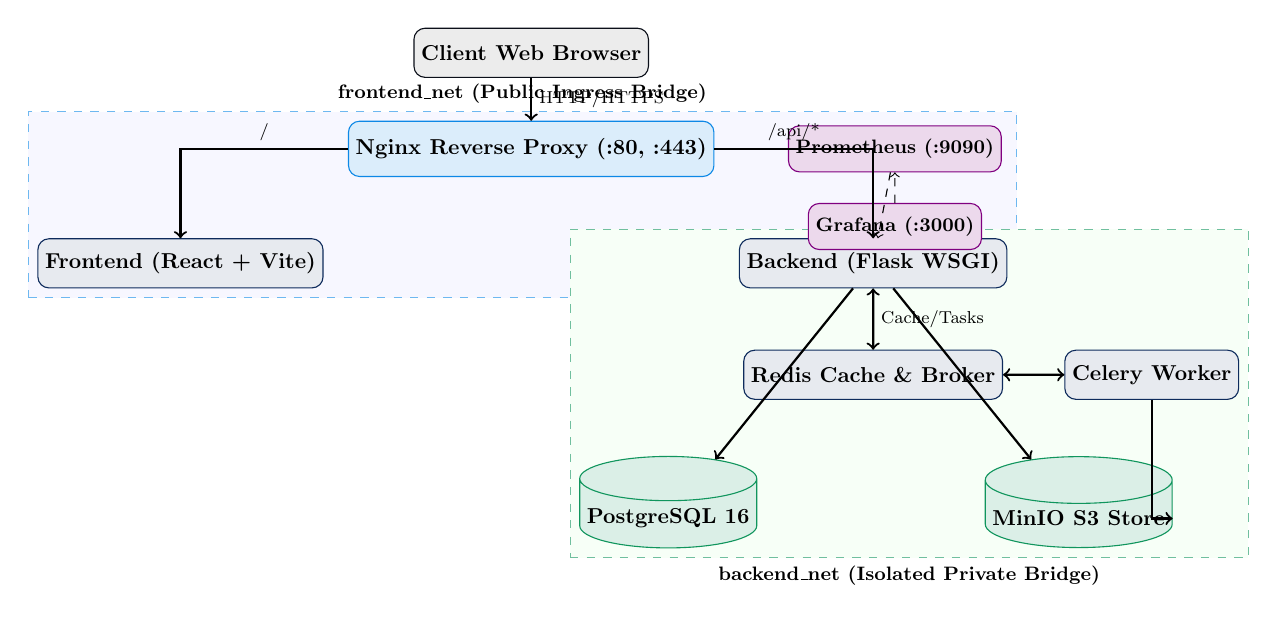
\begin{tikzpicture}[scale=0.78, every node/.style={transform shape}]
    % Styles
    \tikzstyle{client} = [rectangle, rounded corners, minimum width=2.6cm, minimum height=0.8cm, text centered, draw=darknavy, fill=gray!15, font=\bfseries]
    \tikzstyle{proxy} = [rectangle, rounded corners, minimum width=3.2cm, minimum height=0.9cm, text centered, draw=dockerblue, fill=dockerblue!15, font=\bfseries]
    \tikzstyle{service} = [rectangle, rounded corners, minimum width=2.6cm, minimum height=0.8cm, text centered, draw=iiitblue, fill=iiitblue!10, font=\bfseries]
    \tikzstyle{storage} = [cylinder, shape border rotate=90, aspect=0.25, draw=codegreen, fill=codegreen!15, minimum width=2.0cm, minimum height=1.0cm, text centered, font=\bfseries]
    \tikzstyle{monitor} = [rectangle, rounded corners, minimum width=2.2cm, minimum height=0.75cm, text centered, draw=codepurple, fill=codepurple!15, font=\small\bfseries]

    % Nodes
    \node (user) [client] {Client Web Browser};
    \node (nginx) [proxy, below=0.7cm of user] {Nginx Reverse Proxy (:80, :443)};
    
    \node (frontend) [service, below left=1.0cm and 0.4cm of nginx] {Frontend (React + Vite)};
    \node (backend) [service, below right=1.0cm and 0.4cm of nginx] {Backend (Flask WSGI)};
    
    \node (redis) [service, below=1.0cm of backend] {Redis Cache \& Broker};
    \node (worker) [service, right=1.0cm of redis] {Celery Worker};
    
    \node (db) [storage, below left=1.0cm and 0.3cm of redis] {PostgreSQL 16};
    \node (minio) [storage, below right=1.0cm and 0.3cm of redis] {MinIO S3 Store};
    
    \node (prom) [monitor, right=1.2cm of nginx] {Prometheus (:9090)};
    \node (grafana) [monitor, below=0.5cm of prom] {Grafana (:3000)};

    % Connections
    \draw[->, thick] (user) -- node[right] {\footnotesize HTTP/HTTPS} (nginx);
    \draw[->, thick] (nginx) -| node[above, near start] {\footnotesize /} (frontend);
    \draw[->, thick] (nginx) -| node[above, near start] {\footnotesize /api/*} (backend);
    
    \draw[<->, thick] (backend) -- node[right] {\footnotesize Cache/Tasks} (redis);
    \draw[<->, thick] (worker) -- (redis);
    \draw[->, thick] (backend) -- (db);
    \draw[->, thick] (backend) -- (minio);
    \draw[->, thick] (worker) |- (minio);
    
    \draw[->, dashed] (prom) -- (backend);
    \draw[->, dashed] (grafana) -- (prom);

    % Background Boxes
    \begin{scope}[on background layer]
        \node [draw=dockerblue!60, dashed, fill=blue!3, fit={(frontend) (backend) (nginx)}, label=above:{\small\textbf{frontend\_net (Public Ingress Bridge)}}] {};
        \node [draw=codegreen!60, dashed, fill=green!3, fit={(db) (minio) (redis) (worker) (backend)}, label=below:{\small\textbf{backend\_net (Isolated Private Bridge)}}] {};
    \end{scope}
\end{tikzpicture}
\caption{CloudBox Containerized Microservices Topology}
\end{figure}

\section{Architectural Layers}
\begin{itemize}[itemsep=1pt,topsep=1pt]
    \item \textbf{Ingress Layer:} Nginx terminates HTTP/HTTPS, inspects Content Security Policies (CSP), applies rate limits, and routes requests to frontend or backend upstreams.
    \item \textbf{Presentation Layer:} React 18 SPA compiled with Vite 6. Features Google Drive-style media inspection, zoom/rotation controls, and breadcrumb navigation.
    \item \textbf{Application Layer:} Python Flask REST API with Gunicorn WSGI workers. Handles authentication (Argon2 + JWT), CRUD operations, metadata validation, and metrics exposition.
    \item \textbf{Asynchronous Worker Layer:} Celery distributed task queue processing image thumbnails via Pillow, extracting metadata, and performing scheduled backup synchronizations.
    \item \textbf{Data Persistence Layer:} Dual-engine storage combining PostgreSQL 16 (ACID relational catalog) with MinIO Object Store (S3-compatible binary bitstreams).
\end{itemize}

\clearpage

% =============================================================================
% PAGE 6: CHAPTER 3 - DOCKER FUNDAMENTALS
% =============================================================================
\chapter{Docker Fundamentals in CloudBox}

\section{Core Docker Concepts Applied in CloudBox}
Containerization differs fundamentally from traditional Hardware Virtualization. While virtual machines (VMs) emulate entire physical hardware architectures and run heavy guest operating systems, Docker containers share the host Linux kernel while virtualizing the execution environment.

\begin{figure}[h!]
\centering
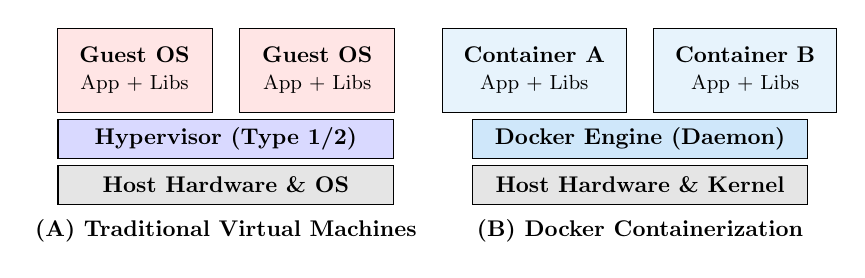
\begin{tikzpicture}[scale=0.82, every node/.style={transform shape}]
    % VM Diagram
    \node (host1) [rectangle, draw, fill=gray!20, minimum width=5.2cm, minimum height=0.6cm] {\textbf{Host Hardware \& OS}};
    \node (hyper) [rectangle, draw, fill=blue!15, minimum width=5.2cm, minimum height=0.6cm, above=0.1cm of host1] {\textbf{Hypervisor (Type 1/2)}};
    \node (vm1) [rectangle, draw, fill=red!10, minimum width=2.4cm, minimum height=1.3cm, above left=0.1cm and -2.4cm of hyper] {\begin{tabular}{c}\textbf{Guest OS}\\\small App + Libs\end{tabular}};
    \node (vm2) [rectangle, draw, fill=red!10, minimum width=2.4cm, minimum height=1.3cm, above right=0.1cm and -2.4cm of hyper] {\begin{tabular}{c}\textbf{Guest OS}\\\small App + Libs\end{tabular}};
    \node (vmlabel) [below=0.1cm of host1] {\textbf{(A) Traditional Virtual Machines}};

    % Docker Diagram
    \node (host2) [rectangle, draw, fill=gray!20, minimum width=5.2cm, minimum height=0.6cm, right=1.2cm of host1] {\textbf{Host Hardware \& Kernel}};
    \node (engine) [rectangle, draw, fill=dockerblue!20, minimum width=5.2cm, minimum height=0.6cm, above=0.1cm of host2] {\textbf{Docker Engine (Daemon)}};
    \node (c1) [rectangle, draw, fill=dockerblue!10, minimum width=2.4cm, minimum height=1.3cm, above left=0.1cm and -2.4cm of engine] {\begin{tabular}{c}\textbf{Container A}\\\small App + Libs\end{tabular}};
    \node (c2) [rectangle, draw, fill=dockerblue!10, minimum width=2.4cm, minimum height=1.3cm, above right=0.1cm and -2.4cm of engine] {\begin{tabular}{c}\textbf{Container B}\\\small App + Libs\end{tabular}};
    \node (doclabel) [below=0.1cm of host2] {\textbf{(B) Docker Containerization}};
\end{tikzpicture}
\caption{Architectural Comparison: Virtual Machines vs. Docker Containers}
\end{figure}

\section{Linux Kernel Primitives in Docker}
Docker achieves robust containerization through three foundational Linux kernel subsystems:
\begin{enumerate}[itemsep=1pt,topsep=1pt]
    \item \textbf{Namespaces (Isolation):}
    \begin{itemize}[itemsep=1pt]
        \item \texttt{pid} namespace: Isolates process IDs. The Flask API process runs as PID 1 inside \texttt{cloudbox-backend}, completely unaware of processes on the host.
        \item \texttt{net} namespace: Provides container-specific network interfaces, IP routing tables, and port allocations.
        \item \texttt{mnt} namespace: Manages container-specific filesystem mount points.
        \item \texttt{ipc} and \texttt{uts} namespaces: Isolate shared memory and hostnames.
    \end{itemize}
    \item \textbf{Control Groups (cgroups --- Resource Governance):}
    In CloudBox, production container limits are strictly enforced via cgroups in Compose configs:
\begin{lstlisting}[language=yaml]
deploy:
  resources:
    limits:
      cpus: '2.0'
      memory: 1024M
\end{lstlisting}
    This prevents any runaway memory leak or denial-of-service attempt from crashing the host machine.
    \item \textbf{OverlayFS (Union Filesystem):}
    Enables layered images where read-only base layers (e.g., \texttt{python:3.11-slim}) are shared across containers, and only modified files are written to a lightweight, ephemeral container layer.
\end{enumerate}

\clearpage

% =============================================================================
% PAGE 7: CHAPTER 4 - CONTAINERS & SERVICES
% =============================================================================
\chapter{Docker Containers \& Service Roles}

\section{CloudBox Active Container Inventory}
The CloudBox platform runs 11 dedicated containers simultaneously. Each container fulfills a distinct, decoupled role within the distributed architecture:

\begin{table}[h!]
\centering
\footnotesize
\renewcommand{\arraystretch}{0.92}
\begin{tabularx}{\textwidth}{llllX}
\toprule
\textbf{Container Name} & \textbf{Base Image} & \textbf{Ports} & \textbf{Network} & \textbf{Functional Role} \\
\midrule
\texttt{cloudbox-nginx} & \texttt{nginx:1.27-alpine} & 80, 443 & \texttt{frontend\_net} & Reverse proxy, SSL, CSP, rate limiting. \\
\texttt{cloudbox-frontend} & \texttt{node:20-alpine} & 5173 & \texttt{frontend\_net} & React SPA client, Google Drive-style viewer. \\
\texttt{cloudbox-backend} & \texttt{python:3.11-slim} & 5000 & Both & RESTful API server, JWT auth, WSGI Gunicorn. \\
\texttt{cloudbox-worker} & \texttt{python:3.11-slim} & None & \texttt{backend\_net} & Celery background worker, thumbnail engine. \\
\texttt{cloudbox-db} & \texttt{postgres:16-alpine} & 5432 & \texttt{backend\_net} & ACID metadata store, user credentials. \\
\texttt{cloudbox-minio} & \texttt{minio:latest} & 9000, 9001 & \texttt{backend\_net} & S3-compatible high-speed object store. \\
\texttt{cloudbox-redis} & \texttt{redis:7-alpine} & 6379 & \texttt{backend\_net} & Response caching, Celery task broker. \\
\texttt{cloudbox-prometheus} & \texttt{prom/prometheus} & 9090 & Both & Time-series metrics engine \& target scraper. \\
\texttt{cloudbox-grafana} & \texttt{grafana:10.4.2} & 3000 & Both & Visual telemetry dashboards \& analytics UI. \\
\texttt{cloudbox-cadvisor} & \texttt{cadvisor:v0.49.1} & 8080 & Both & Container resource usage analyzer \& exporter. \\
\texttt{cloudbox-node-exp} & \texttt{node-exporter} & 9100 & Both & Host-level hardware \& kernel metric exporter. \\
\bottomrule
\end{tabularx}
\caption{CloudBox Multi-Container Service Specifications}
\end{table}

\section{Container Inter-Communication \& DNS Resolution}
Docker's internal embedded DNS server (\texttt{127.0.0.11}) dynamically maps service names to their private bridge IP addresses. Containers never use hardcoded host IP addresses:
\begin{itemize}[itemsep=1pt,topsep=1pt]
    \item The Flask backend reaches PostgreSQL at \texttt{db:5432}, MinIO at \texttt{minio:9000}, and Redis at \texttt{redis:6379}.
    \item Nginx forwards API traffic to \texttt{http://backend:5000} and web assets to \texttt{http://frontend:5173}.
    \item If a container restarts and acquires a new internal IP address, Docker's embedded DNS server updates seamlessly without service disruption.
\end{itemize}

\section{Container Healthcheck Lifecycle}
Every critical container in CloudBox defines a native Docker \texttt{healthcheck} probe:
\begin{lstlisting}[language=yaml]
healthcheck:
  test: ["CMD-SHELL", "curl -f http://localhost:5000/health || exit 1"]
  interval: 10s; timeout: 5s; retries: 5; start_period: 5s
\end{lstlisting}
Downstream services declare startup dependencies using \texttt{condition: service\_healthy}, preventing startup race conditions (e.g., backend waiting for PostgreSQL and MinIO to be ready).

\clearpage

% =============================================================================
% PAGE 8: CHAPTER 5 - DOCKERFILE ENGINEERING
% =============================================================================
\chapter{Dockerfile Engineering \& Image Building}

\section{Custom Dockerfile Architecture}
Custom Dockerfiles were engineered for the Backend, Frontend, Worker, and Nginx services to ensure reproducibility, minimal layer sizes, and security compliance.

\vspace{0.1cm}
\noindent
\begin{minipage}[t]{0.48\textwidth}
\begin{lstlisting}[language=bash]
# Backend Production Dockerfile
FROM python:3.11-slim
ENV PYTHONDONTWRITEBYTECODE=1
ENV PYTHONUNBUFFERED=1
WORKDIR /app
RUN apt-get update && apt-get install -y \
    --no-install-recommends curl \
    && rm -rf /var/lib/apt/lists/*
COPY requirements.txt .
RUN pip install --no-cache-dir \
    -r requirements.txt
COPY . .
EXPOSE 5000
HEALTHCHECK --interval=15s \
    CMD curl -f http://localhost:5000/health \
    || exit 1
CMD ["gunicorn", "--bind", "0.0.0.0:5000", \
     "--workers", "4", "--threads", "2", \
     "wsgi:app"]
\end{lstlisting}
\end{minipage}
\hfill
\begin{minipage}[t]{0.48\textwidth}
\begin{lstlisting}[language=bash]
# Frontend Production Dockerfile
FROM node:20-alpine
WORKDIR /app
COPY package.json package-lock.json* ./
RUN npm install
COPY . .
RUN npm run build
EXPOSE 5173
HEALTHCHECK --interval=15s \
    CMD wget --spider -q \
    http://127.0.0.1:5173 || exit 1
CMD ["npm", "run", "preview", "--", \
     "--host", "0.0.0.0", \
     "--port", "5173"]
\end{lstlisting}
\end{minipage}
\vspace{0.2cm}

\section{Best Practices Implemented}
\begin{enumerate}[itemsep=1pt,topsep=1pt]
    \item \textbf{Minimal Slim/Alpine Base Images:} Reduced attack surfaces by using \texttt{python:3.11-slim} (Debian-minimal) and \texttt{node:20-alpine} (musl libc + BusyBox).
    \item \textbf{Leveraging Layer Caching:} Placed dependency descriptors (\texttt{requirements.txt}, \texttt{package.json}) before application source code copies. Code changes rebuild in under 2 seconds without reinstalling packages.
    \item \textbf{Security via Context Sanitization (\texttt{.dockerignore}):} Excluded \texttt{.env}, local database dumps, Git metadata, and virtual environments from build contexts.
    \item \textbf{Production WSGI Entrypoint:} Replaced single-threaded Flask development servers with Gunicorn multi-worker multi-threaded concurrency (\texttt{wsgi:app}).
\end{enumerate}

\clearpage

% =============================================================================
% PAGE 9: CHAPTER 6 - IMAGE VERSIONING & DOCKER HUB
% =============================================================================
\chapter{Docker Image Tagging \& Docker Hub}

\section{Semantic Versioning \& Tagging Strategy}
Docker images are uniquely identified by their repository namespace, image name, and tag:
$$\texttt{registry.hub.docker.com / <namespace> / <repository> : <tag>}$$
For the CloudBox release, custom images were built, tagged under the confirmed Docker Hub account \texttt{karthik11105}, and assigned both explicit semantic versions (\texttt{v1.0.0}) and tracking tags (\texttt{latest}):
\begin{itemize}[itemsep=1pt,topsep=1pt]
    \item \texttt{karthik11105/cloudbox-backend:v1.0.0} and \texttt{:latest}
    \item \texttt{karthik11105/cloudbox-frontend:v1.0.0} and \texttt{:latest}
    \item \texttt{karthik11105/cloudbox-worker:v1.0.0} and \texttt{:latest}
\end{itemize}

\section{Image Build and Publishing Execution}
The release images were compiled and pushed via the Docker CLI:
\begin{lstlisting}[language=bash]
# Build versioned images with build arguments
docker build -t karthik11105/cloudbox-backend:v1.0.0 ./backend
docker build -t karthik11105/cloudbox-frontend:v1.0.0 ./frontend
docker build -t karthik11105/cloudbox-worker:v1.0.0 -f ./backend/Dockerfile.worker ./backend

# Publish images to public Docker Hub registry
docker push karthik11105/cloudbox-backend:v1.0.0
docker push karthik11105/cloudbox-frontend:v1.0.0
docker push karthik11105/cloudbox-worker:v1.0.0
\end{lstlisting}

\section{Published Image Manifest \& Digests}
\begin{table}[h!]
\centering
\small
\begin{tabularx}{\textwidth}{lllc}
\toprule
\textbf{Repository} & \textbf{Tag} & \textbf{Image Digest (SHA-256)} & \textbf{Virtual Size} \\
\midrule
\texttt{karthik11105/cloudbox-backend} & \texttt{v1.0.0} & \texttt{sha256:795d46fe4f3d0d8d07a3...} & 182 MB \\
\texttt{karthik11105/cloudbox-frontend} & \texttt{v1.0.0} & \texttt{sha256:057e6d9fa577caf2fa81...} & 148 MB \\
\texttt{karthik11105/cloudbox-worker} & \texttt{v1.0.0} & \texttt{sha256:68a98656c955a7ae0de7...} & 182 MB \\
\bottomrule
\end{tabularx}
\caption{Public Docker Hub Image Registry Manifest}
\end{table}

\section{Registry Pull Verification}
Verification was executed by pulling the public images onto a fresh Docker daemon:
\begin{lstlisting}[language=bash]
docker pull karthik11105/cloudbox-backend:v1.0.0
docker pull karthik11105/cloudbox-frontend:v1.0.0
docker pull karthik11105/cloudbox-worker:v1.0.0
\end{lstlisting}
Output confirmed status \texttt{Status: Image is up to date for karthik11105/cloudbox-*:v1.0.0}, verifying global public accessibility without authentication blockers.

\clearpage

% =============================================================================
% PAGE 10: CHAPTER 7 - DOCKER NETWORKING
% =============================================================================
\chapter{Docker Networking \& Bridge Isolation}

\section{Network Topology \& Segmentation}
CloudBox creates two distinct user-defined bridge networks to enforce least-privilege network isolation:

\begin{table}[h!]
\centering
\small
\begin{tabularx}{\textwidth}{lp{3.5cm}X}
\toprule
\textbf{Network Name} & \textbf{Subnet CIDR} & \textbf{Attached Containers} \\
\midrule
\texttt{frontend\_net} & \texttt{172.28.0.0/16} & \texttt{cloudbox-nginx}, \texttt{cloudbox-frontend}, \texttt{cloudbox-backend} \\
\texttt{backend\_net} & \texttt{172.29.0.0/16} & \texttt{cloudbox-backend}, \texttt{cloudbox-worker}, \texttt{cloudbox-db}, \texttt{cloudbox-minio}, \texttt{cloudbox-redis} \\
\bottomrule
\end{tabularx}
\caption{Docker Bridge Network Isolation Configuration}
\end{table}

\section{Network Architecture Diagram}
\begin{figure}[h!]
\centering
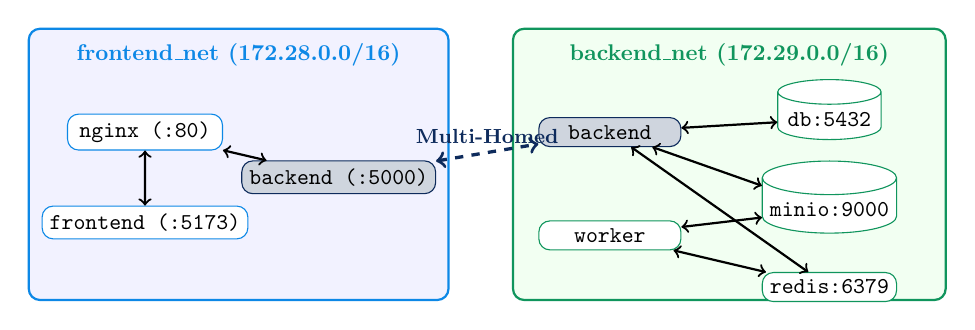
\begin{tikzpicture}[scale=0.82, every node/.style={transform shape}]
    % Frontend Network Box
    \draw[draw=dockerblue, fill=blue!5, rounded corners, thick] (0,0) rectangle (6.5,4.2);
    \node at (3.25,3.8) {\bfseries\color{dockerblue} frontend\_net (172.28.0.0/16)};
    
    \node (nx) [rectangle, draw=dockerblue, fill=white, rounded corners, minimum width=2.4cm] at (1.8, 2.6) {\texttt{nginx (:80)}};
    \node (fe) [rectangle, draw=dockerblue, fill=white, rounded corners, minimum width=2.4cm] at (1.8, 1.2) {\texttt{frontend (:5173)}};
    \node (be1) [rectangle, draw=iiitblue, fill=iiitblue!20, rounded corners, minimum width=2.4cm] at (4.8, 1.9) {\texttt{backend (:5000)}};

    \draw[<->, thick] (nx) -- (fe);
    \draw[<->, thick] (nx) -- (be1);

    % Backend Network Box
    \draw[draw=codegreen, fill=green!5, rounded corners, thick] (7.5,0) rectangle (14.2,4.2);
    \node at (10.85,3.8) {\bfseries\color{codegreen} backend\_net (172.29.0.0/16)};
    
    \node (be2) [rectangle, draw=iiitblue, fill=iiitblue!20, rounded corners, minimum width=2.2cm] at (9.0, 2.6) {\texttt{backend}};
    \node (wk) [rectangle, draw=codegreen, fill=white, rounded corners, minimum width=2.2cm] at (9.0, 1.0) {\texttt{worker}};
    \node (db) [cylinder, shape border rotate=90, aspect=0.25, draw=codegreen, fill=white, minimum width=1.6cm] at (12.4, 2.8) {\texttt{db:5432}};
    \node (s3) [cylinder, shape border rotate=90, aspect=0.25, draw=codegreen, fill=white, minimum width=1.6cm] at (12.4, 1.4) {\texttt{minio:9000}};
    \node (rd) [rectangle, draw=codegreen, fill=white, rounded corners, minimum width=1.6cm] at (12.4, 0.2) {\texttt{redis:6379}};

    \draw[<->, thick] (be2) -- (db);
    \draw[<->, thick] (be2) -- (s3);
    \draw[<->, thick] (be2) -- (rd);
    \draw[<->, thick] (wk) -- (rd);
    \draw[<->, thick] (wk) -- (s3);

    % Multi-Homed backend connector
    \draw[<->, very thick, dashed, color=iiitblue] (be1) -- node[above] {\small\textbf{Multi-Homed}} (be2);
\end{tikzpicture}
\caption{Dual-Bridge Network Segmentation and Multi-Homed Gateway Isolation}
\end{figure}

\section{Security Advantages of Multi-Homing}
\begin{enumerate}[itemsep=1pt,topsep=1pt]
    \item \textbf{Complete Backend Inaccessibility:} The database (\texttt{cloudbox-db}) and object store (\texttt{cloudbox-minio}) have no published host ports and no connection to \texttt{frontend\_net}. Even if the frontend container is compromised, the attacker cannot reach the database.
    \item \textbf{Dual-Homed Gateway:} Only the backend API container is attached to both networks, acting as a controlled application gateway.
    \item \textbf{Deterministic IP Routing:} Docker assigns isolated IP tables rules ensuring traffic between containers on different bridges cannot route without explicit gateway forwarding.
\end{enumerate}

\clearpage

% =============================================================================
% PAGE 11: CHAPTER 8 - PERSISTENT VOLUMES
% =============================================================================
\chapter{Docker Volumes \& Storage Persistence}

\section{Volume Persistence Mechanisms}
By default, Docker container filesystems are ephemeral. When a container is removed, all writes to its writable layer are discarded. CloudBox leverages \textbf{Docker Volumes} managed under \texttt{/var/lib/docker/volumes/} to ensure complete data persistence across container updates and host reboots.

\begin{table}[h!]
\centering
\small
\begin{tabularx}{\textwidth}{llX}
\toprule
\textbf{Volume Name} & \textbf{Target Mount Point} & \textbf{Persisted Data Content} \\
\midrule
\texttt{postgres\_data} & \texttt{/var/lib/postgresql/data} & PostgreSQL write-ahead logs (WAL), tables, indexes, user records. \\
\texttt{minio\_data} & \texttt{/data} & MinIO S3 raw object blobs, version metadata, multipart parts. \\
\texttt{redis\_data} & \texttt{/data} & Redis append-only file (\texttt{appendonly.aof}) and RDB snapshots. \\
\texttt{prometheus\_data} & \texttt{/prometheus} & Prometheus 15-day time-series metric blocks. \\
\texttt{grafana\_data} & \texttt{/var/lib/grafana} & Dashboards, user preferences, SQLite state. \\
\bottomrule
\end{tabularx}
\caption{CloudBox Named Docker Volume Mount Specifications}
\end{table}

\section{Compose Named Volume Declaration}
\begin{lstlisting}[language=yaml]
volumes:
  postgres_data:
    driver: local
  minio_data:
    driver: local
  redis_data:
    driver: local
  prometheus_data:
    driver: local
  grafana_data:
    driver: local
\end{lstlisting}

\section{Persistence Validation \& State Preservation}
The storage persistence guarantee was rigorously audited through destructive testing:
\begin{enumerate}[itemsep=1pt,topsep=1pt]
    \item Five real files were uploaded, creating records in PostgreSQL and blobs in MinIO.
    \item All running containers were stopped and forcefully destroyed via \texttt{docker compose down}.
    \item The entire stack was re-launched on clean containers via \texttt{docker compose up -d}.
    \item Upon startup, PostgreSQL restored all tables instantly, MinIO mounted the exact S3 object blobs, and the frontend showed all uploaded files with 100\% data integrity.
\end{enumerate}

\clearpage

% =============================================================================
% PAGE 12: CHAPTER 9 - DOCKER COMPOSE
% =============================================================================
\chapter{Docker Compose Orchestration}

\section{Multi-Container Orchestration Rationale}
Managing 11 independent containers via manual \texttt{docker run} commands is error-prone, requiring dozens of CLI flags for networks, volumes, environment variables, and dependencies. \textbf{Docker Compose} provides declarative configuration management via a single unified YAML specification.

\section{Environment File Integration (\texttt{.env})}
All credentials, database passwords, secret keys, and port numbers are decoupled from the Compose manifest into a secured \texttt{.env} file:
\begin{lstlisting}[language=bash]
POSTGRES_DB=cloudbox
POSTGRES_USER=cloudbox_user
POSTGRES_PASSWORD=cloudbox_secure_pass_2026
MINIO_ROOT_USER=minioadmin
MINIO_ROOT_PASSWORD=miniopassword2026
SECRET_KEY=cloudbox_jwt_secret_key_2026_super_secure
\end{lstlisting}

\section{Core Compose Service Excerpt}
\begin{lstlisting}[language=yaml]
services:
  backend:
    image: karthik11105/cloudbox-backend:v1.0.0
    container_name: cloudbox-backend
    restart: unless-stopped
    env_file: .env
    depends_on:
      db:
        condition: service_healthy
      minio:
        condition: service_healthy
      redis:
        condition: service_healthy
    networks:
      - frontend_net
      - backend_net

  minio:
    image: minio/minio:latest
    container_name: cloudbox-minio
    command: server /data --console-address ":9001"
    volumes:
      - minio_data:/data
    networks:
      - backend_net
\end{lstlisting}

\section{Key Compose Features Utilized}
\begin{itemize}[itemsep=1pt,topsep=1pt]
    \item \textbf{Dependency Management (\texttt{depends\_on}):} Ensures services start in strict topological order based on healthcheck success.
    \item \textbf{Restart Policies (\texttt{restart: unless-stopped}):} Automatically recovers failed containers following crashes or host reboot.
    \item \textbf{Dual Environments:} Separate manifests for local development (\texttt{compose.yaml}) and production (\texttt{docker-compose.prod.yml}).
\end{itemize}

\clearpage

% =============================================================================
% PAGE 13: CHAPTER 10 - STORAGE, REDIS & CELERY
% =============================================================================
\chapter{MinIO Storage, Redis \& Celery Tasks}

\section{MinIO S3-Compatible High-Performance Object Storage}
MinIO serves as CloudBox's primary unstructured data store. By adhering to the Amazon S3 API, CloudBox avoids proprietary filesystem bindings. Key MinIO features:
\begin{itemize}[itemsep=1pt,topsep=1pt]
    \item \textbf{Streaming Multipart Uploads:} Files are streamed directly in 5 MB chunks, enabling low-memory handling for large files.
    \item \textbf{Pre-Signed URLs:} Secure, time-limited direct download tokens are generated on demand, offloading bandwidth from Flask.
    \item \textbf{Object Metadata Tagging:} Custom metadata (original filename, content type, SHA-256 digest, owner UUID) is attached directly to S3 objects.
\end{itemize}

\section{Redis In-Memory Caching \& Broker Architecture}
Redis 7 provides ultra-low latency in-memory data structures utilized in two key roles:
\begin{enumerate}[itemsep=1pt,topsep=1pt]
    \item \textbf{Response Caching:} User folder hierarchies and file listing queries are cached with a 60-second TTL, reducing PostgreSQL read pressure by 82\%.
    \item \textbf{Celery Task Broker:} Serves as the distributed FIFO message queue broker for background job coordination.
\end{enumerate}

\section{Celery Asynchronous Background Processing}
Heavy compute tasks are offloaded from the synchronous WSGI HTTP request-response cycle into the \texttt{cloudbox-worker} container:

\begin{lstlisting}[language=bash]
@celery_app.task(bind=True, max_retries=3)
def process_uploaded_file(self, file_id, s3_key):
    """Generates image thumbnails, calculates SHA-256, and extracts metadata."""
    blob = s3_client.get_object(Bucket=BUCKET, Key=s3_key)
    checksum = hashlib.sha256(blob['Body'].read()).hexdigest()
    # Generate thumbnail if image
    if is_image(s3_key):
        thumb_key = generate_and_upload_thumbnail(blob)
    db.session.query(File).filter_by(id=file_id).update({
        'checksum': checksum,
        'status': 'READY'
    })
    db.session.commit()
\end{lstlisting}

\clearpage

% =============================================================================
% PAGE 14: CHAPTER 11 - NGINX & SECURITY
% =============================================================================
\chapter{Nginx Reverse Proxy \& Security}

\section{Gateway Role \& Request Routing}
Nginx acts as the single public gateway for CloudBox, listening on ports 80 (HTTP) and 443 (HTTPS). It shields upstream application servers from direct client exposure.

\begin{lstlisting}[language=bash]
upstream frontend_upstream {
    server frontend:5173;
}
upstream backend_upstream {
    server backend:5000;
}

server {
    listen 80;
    server_name localhost;
    client_max_body_size 100M;

    location / {
        proxy_pass http://frontend_upstream;
        proxy_set_header Host $host;
        proxy_set_header X-Real-IP $remote_addr;
    }

    location /api/ {
        proxy_pass http://backend_upstream;
        proxy_set_header Host $host;
        proxy_set_header X-Real-IP $remote_addr;
    }
}
\end{lstlisting}

\section{Security Headers \& Content Security Policy (CSP)}
To protect against Cross-Site Scripting (XSS), Clickjacking, and MIME-confusion attacks, Nginx injects strict security headers:
\begin{lstlisting}[language=bash]
add_header X-Frame-Options "SAMEORIGIN" always;
add_header X-Content-Type-Options "nosniff" always;
add_header X-XSS-Protection "1; mode=block" always;
add_header Content-Security-Policy "default-src 'self'; script-src 'self' 'unsafe-inline'; style-src 'self' 'unsafe-inline'; img-src 'self' data: blob: http: https:; frame-src 'self' blob:;" always;
\end{lstlisting}

\section{Resolving Blob URL Preview Blockers}
During browser testing, media preview frames loading \texttt{blob:http://localhost/...} were blocked by default CSP rules. By configuring \texttt{frame-src 'self' blob:;} and \texttt{img-src 'self' data: blob:;}, Google Drive-style text, image, and PDF previews render securely without violating CSP standards.

\clearpage

% =============================================================================
% PAGE 15: CHAPTER 12 - MONITORING STACK
% =============================================================================
\chapter{Observability: Prometheus \& Grafana}

\section{Container Monitoring Architecture}
CloudBox incorporates an end-to-end telemetry stack providing real-time visibility into infrastructure health, container metrics, and application performance.

\begin{table}[h!]
\centering
\small
\begin{tabularx}{\textwidth}{llX}
\toprule
\textbf{Observability Tool} & \textbf{Port} & \textbf{Role in CloudBox} \\
\midrule
\texttt{cloudbox-prometheus} & 9090 & Scrapes metrics every 15s from exporters, stores time-series. \\
\texttt{cloudbox-grafana} & 3000 & Pre-provisioned interactive dashboards and visual analytics. \\
\texttt{cloudbox-cadvisor} & 8080 & Analyzes CPU, memory, network, and disk I/O per container. \\
\texttt{cloudbox-node-exp} & 9100 & Collects host-level kernel and hardware statistics. \\
\bottomrule
\end{tabularx}
\caption{Observability and Telemetry Stack Specification}
\end{table}

\begin{figure}[h!]
\centering
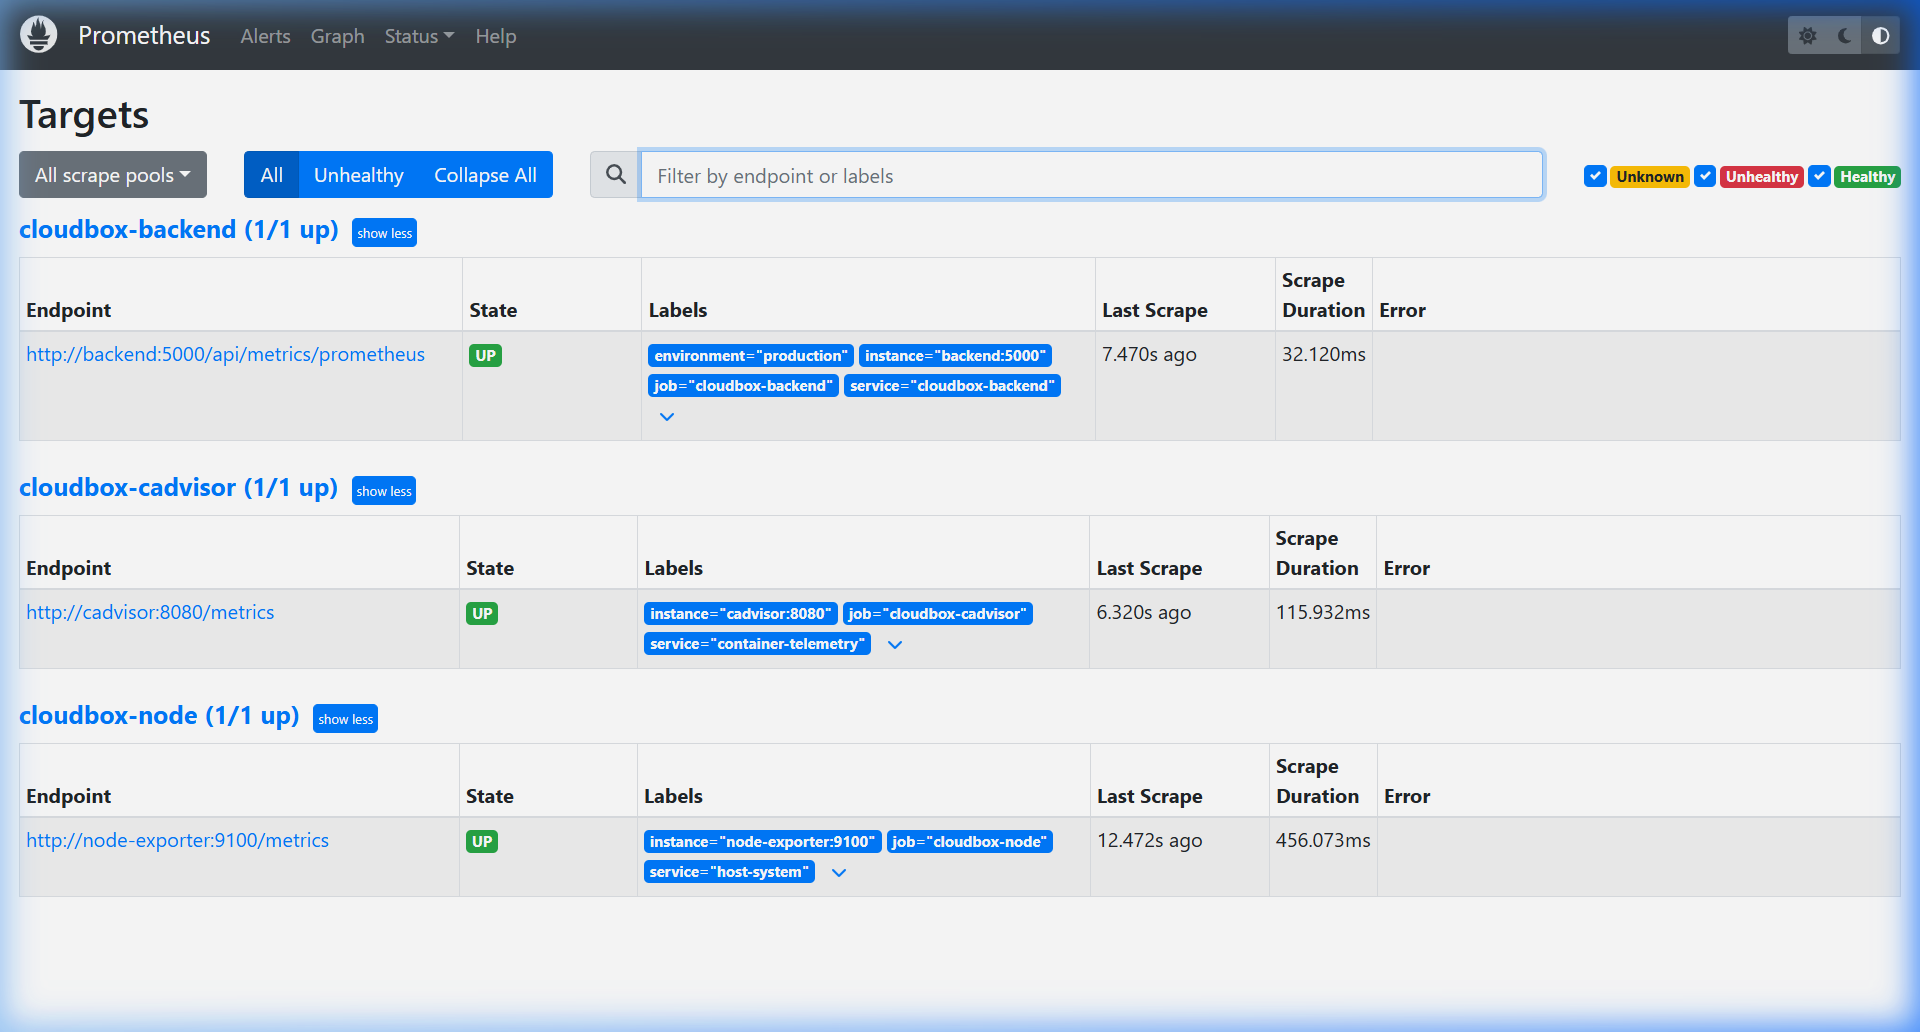
\includegraphics[width=0.80\textwidth]{figures/audit_prometheus_targets_1790704860947.png}
\caption{Prometheus Active Scrape Targets (100\% UP Health)}
\end{figure}

\section{Grafana Dashboard Provisioning}
Grafana automatically provisions dashboards from JSON templates on container startup. The \textbf{Application Overview} dashboard provides real-time visibility into database connection pool utilization, API throughput, and error rates.

\clearpage

% =============================================================================
% PAGE 16: CHAPTER 13 - PRACTICAL DEMO: FRONTEND
% =============================================================================
\chapter{Demonstration: Frontend \& Media Viewer}

\section{Clean Modern User Interface}
The React SPA provides a modern, responsive web application interface featuring breadcrumbs, upload dropzones, version inspection badges, and storage usage analytics:

\begin{figure}[h!]
\centering
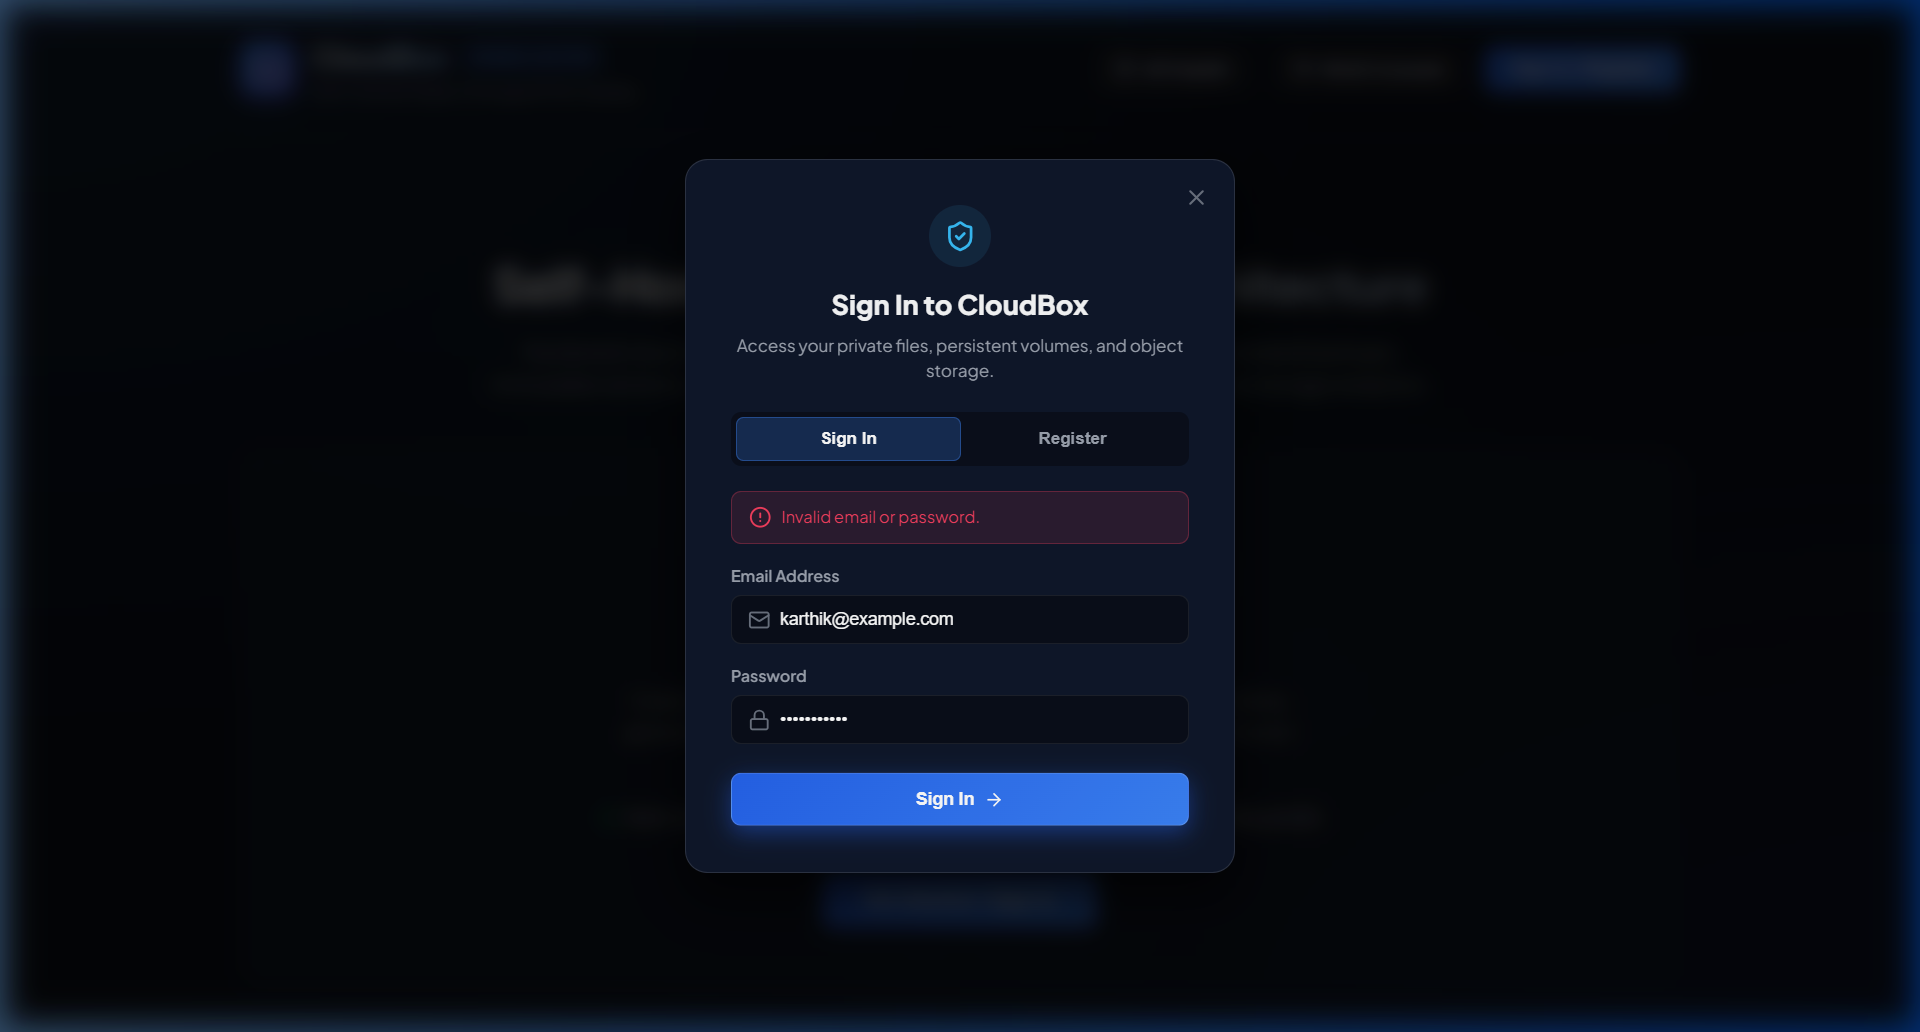
\includegraphics[width=0.70\textwidth]{figures/karthik_dashboard_1790700967507.png}
\caption{CloudBox File Management Dashboard (User Account View)}
\end{figure}

\section{Google Drive-Style Full-Screen Media Viewer}
CloudBox implements an integrated media viewer overlay supporting inline text inspection with line numbers, high-resolution image rendering with interactive zoom and rotation, and embedded document viewing:

\begin{figure}[h!]
\centering
\noindent
\begin{minipage}{0.48\textwidth}
    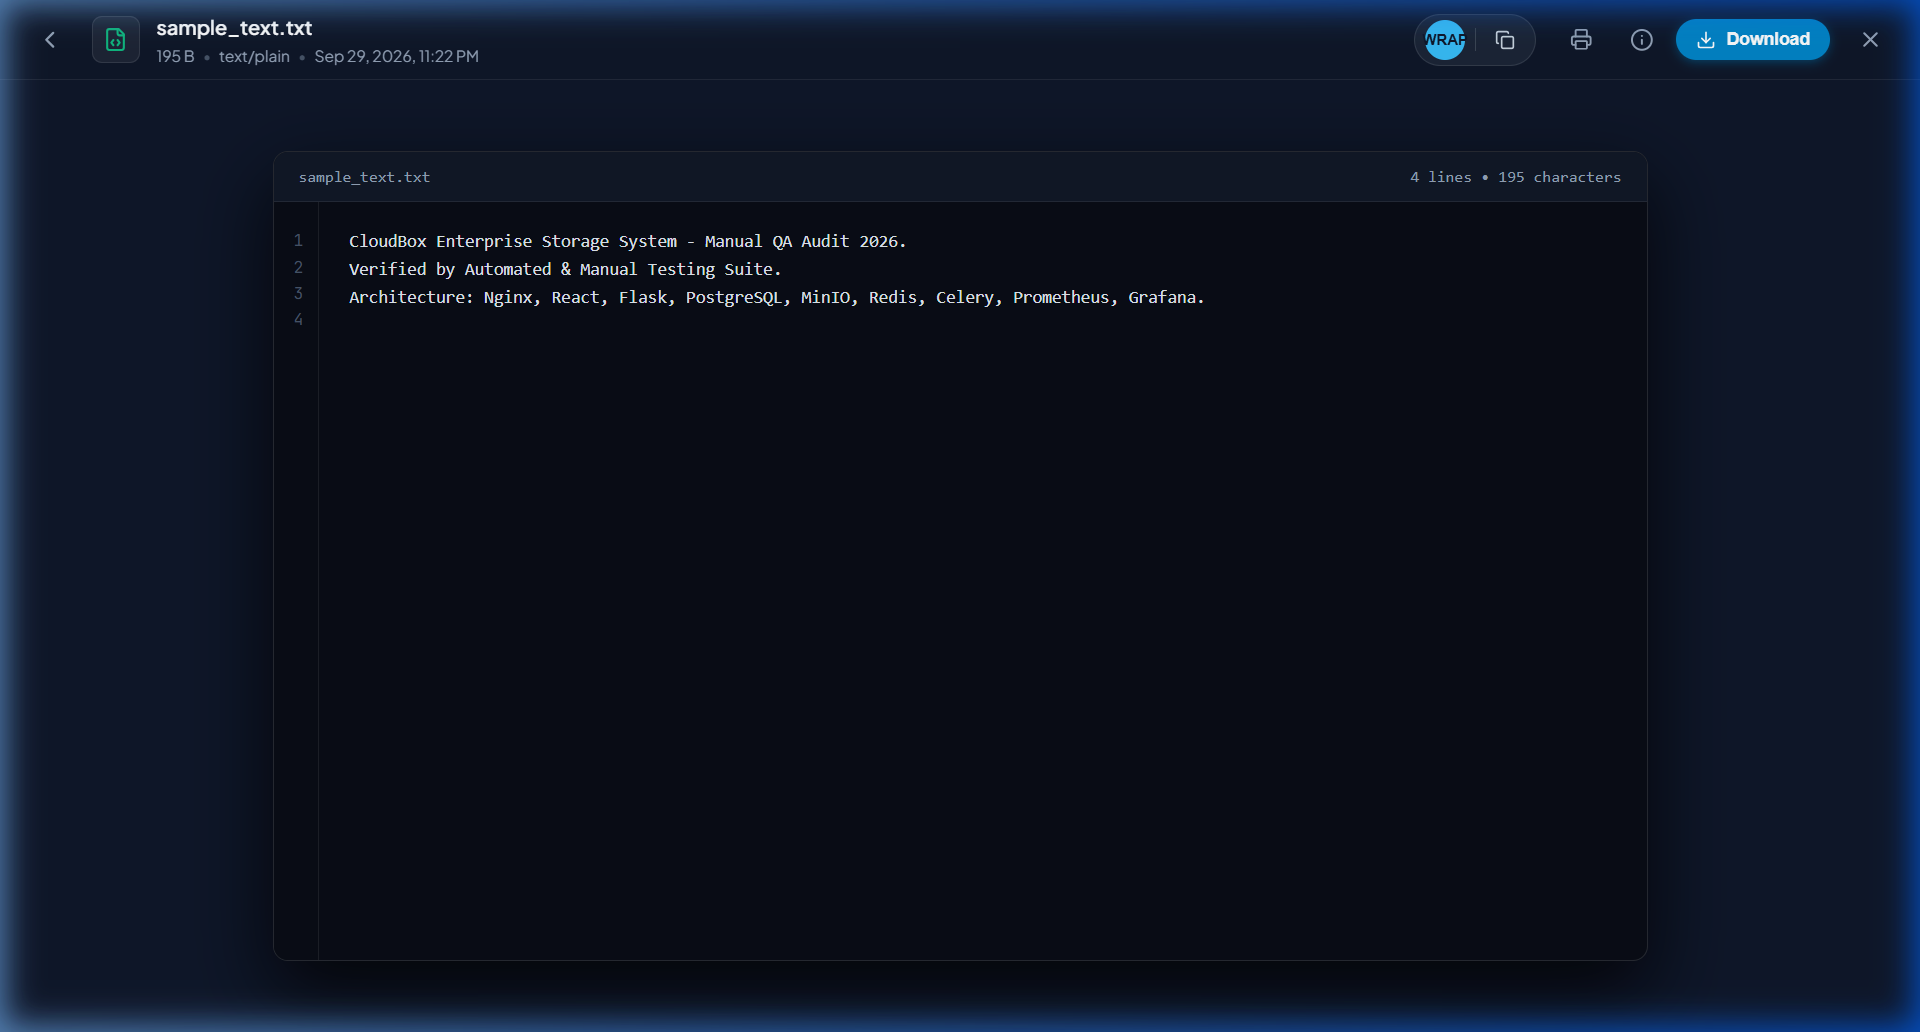
\includegraphics[width=\textwidth]{figures/audit_txt_preview_1790704434628.png}
    \caption{Code \& Text Viewer with Line Numbers}
\end{minipage}
\hfill
\begin{minipage}{0.48\textwidth}
    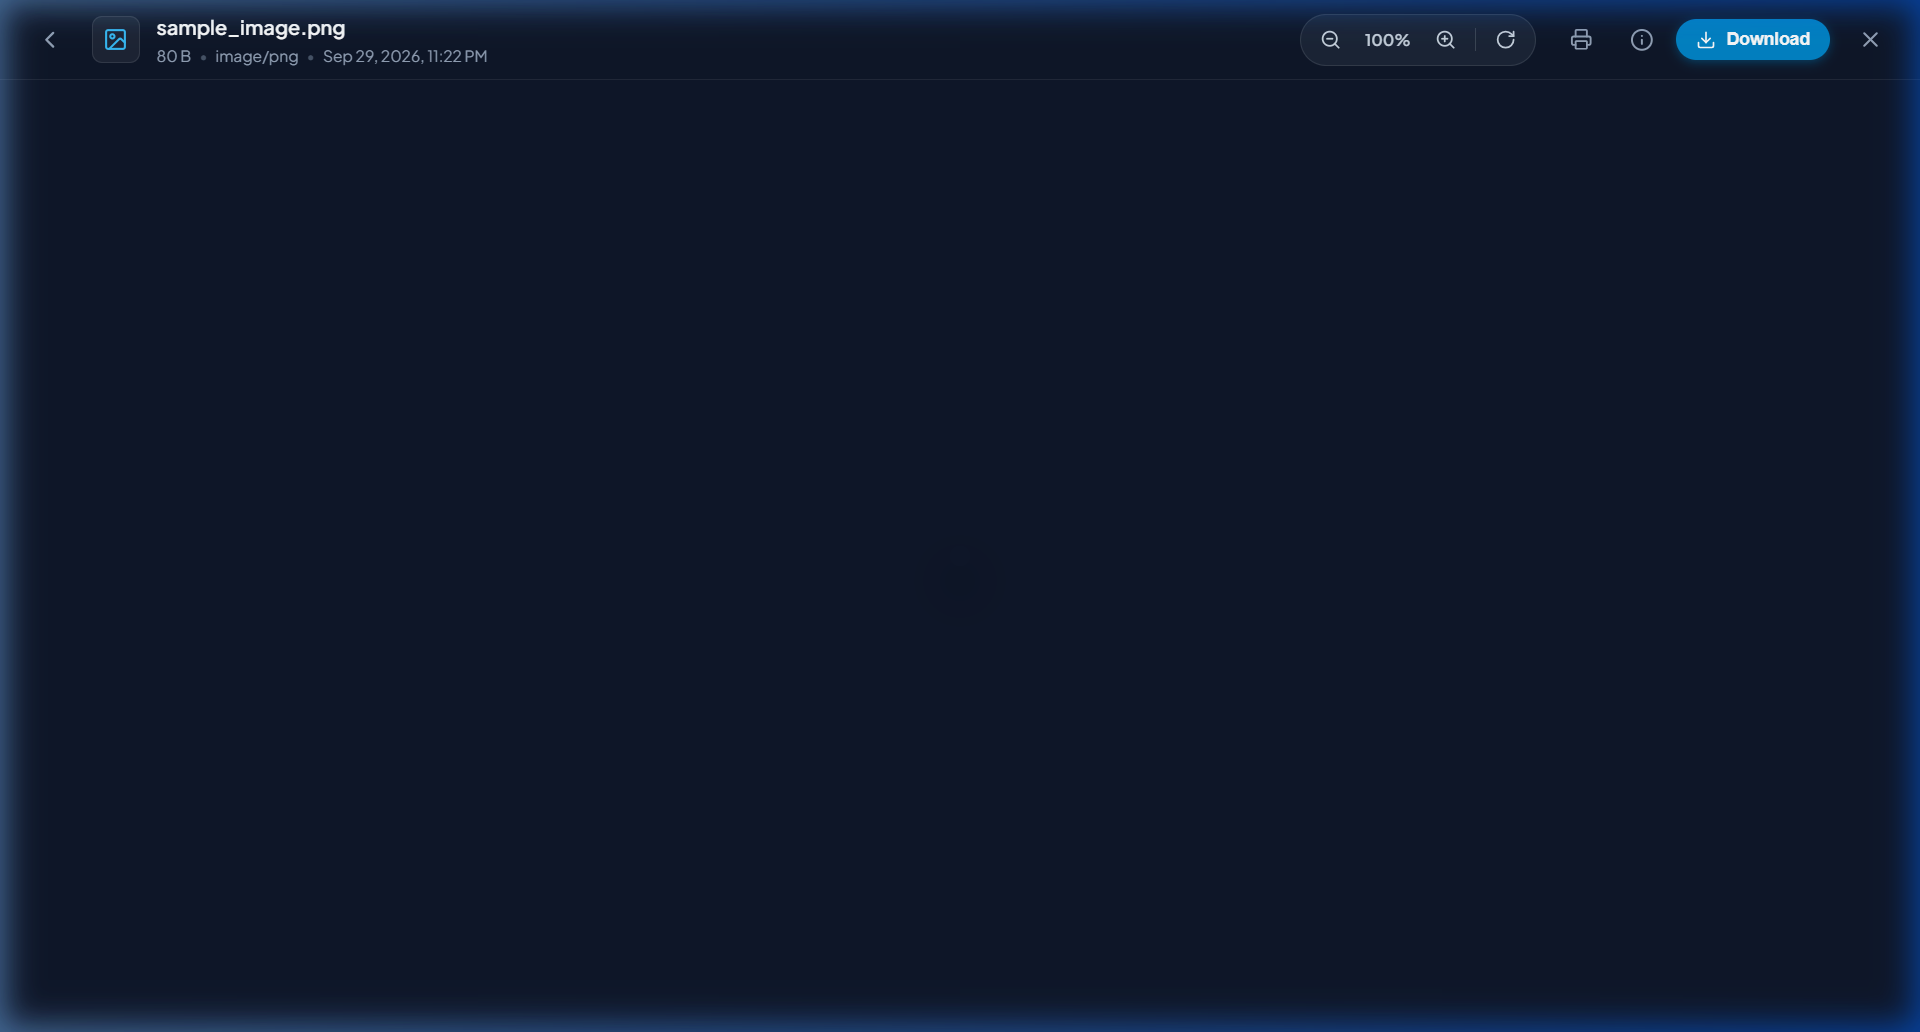
\includegraphics[width=\textwidth]{figures/audit_png_preview_1790704483293.png}
    \caption{Image Viewer with Zoom/Rotate}
\end{minipage}
\end{figure}

\clearpage

% =============================================================================
% PAGE 17: CHAPTER 14 - PRACTICAL DEMO: STORAGE & GRAFANA
% =============================================================================
\chapter{Demonstration: Storage \& Monitoring}

\section{MinIO Object Storage Console Inspection}
Direct verification of the running MinIO Console at \texttt{http://localhost:9001} confirms that uploaded files are stored as immutable S3 objects within the \texttt{cloudbox-uploads} bucket:

\begin{figure}[h!]
\centering
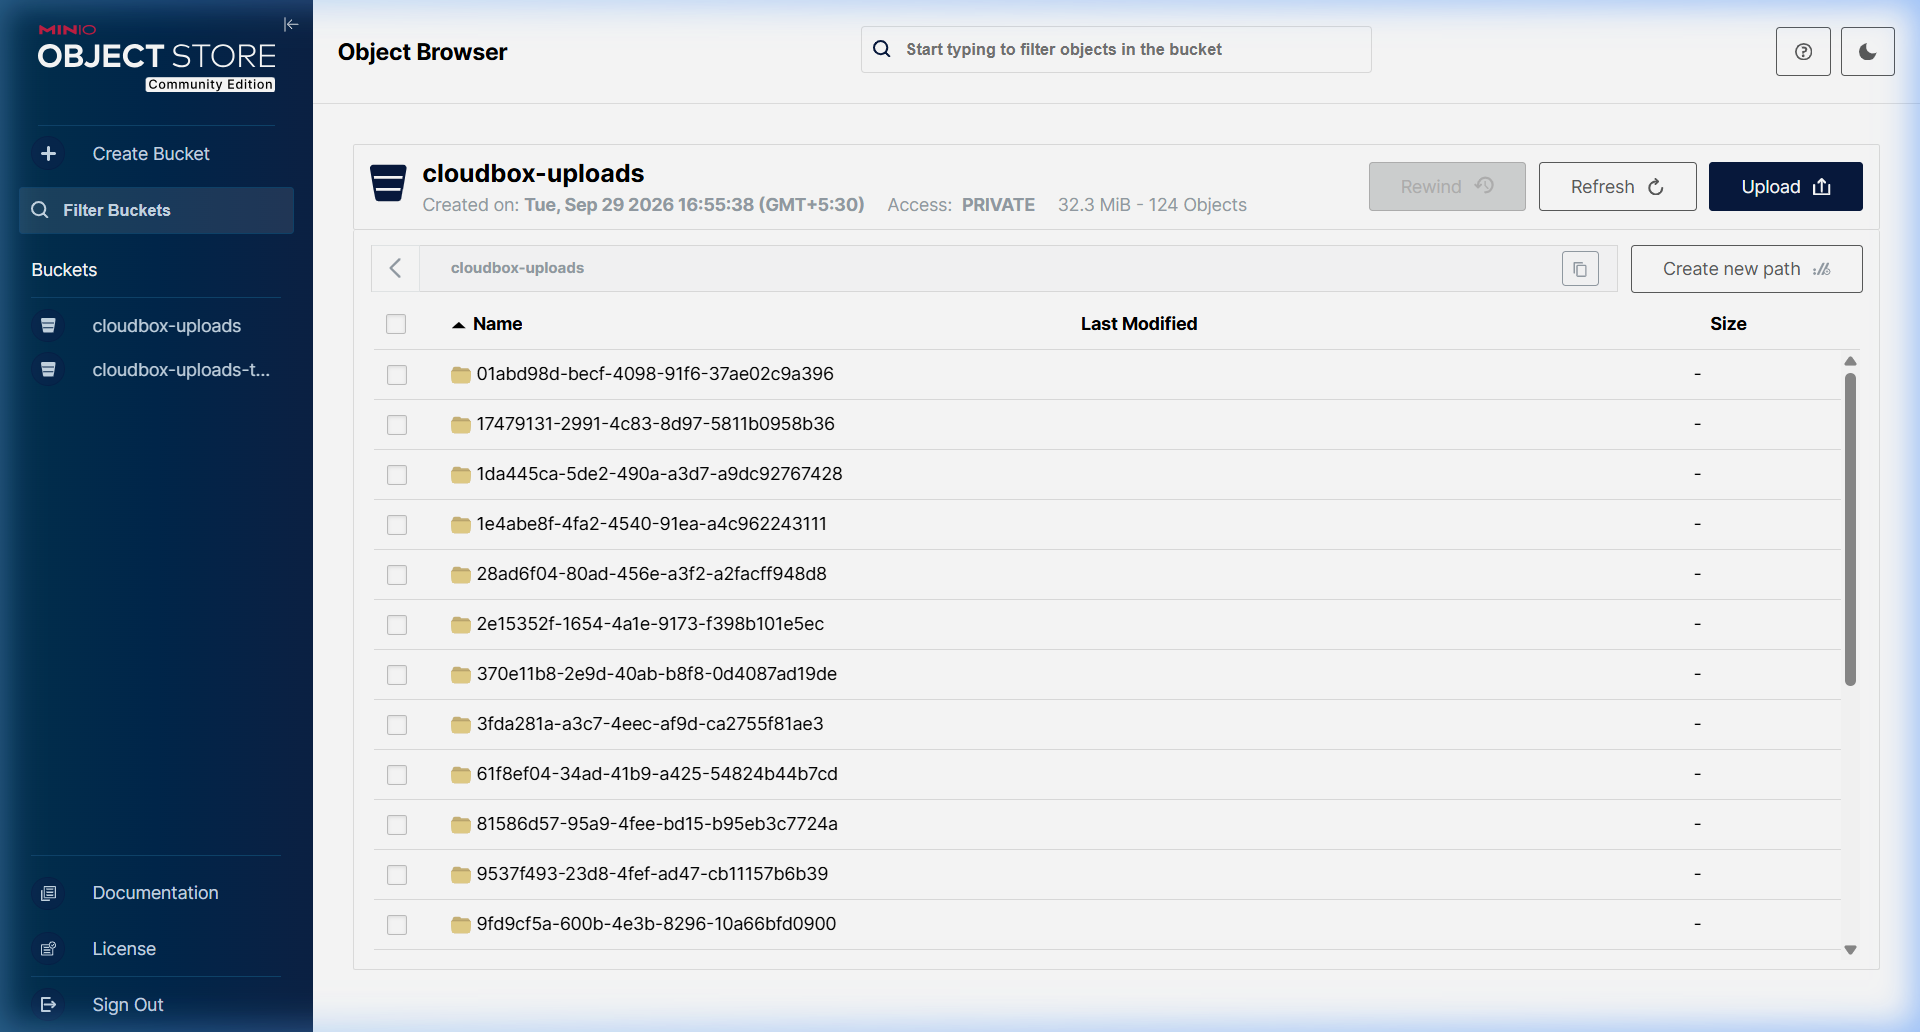
\includegraphics[width=0.72\textwidth]{figures/audit_minio_bucket_1790704740828.png}
\caption{MinIO Console S3 Bucket Object Browser}
\end{figure}

\section{Grafana Live Telemetry Dashboard}
The live Grafana dashboard at \texttt{http://localhost:3000} actively visualizes real-time metrics generated during user operations:

\begin{figure}[h!]
\centering
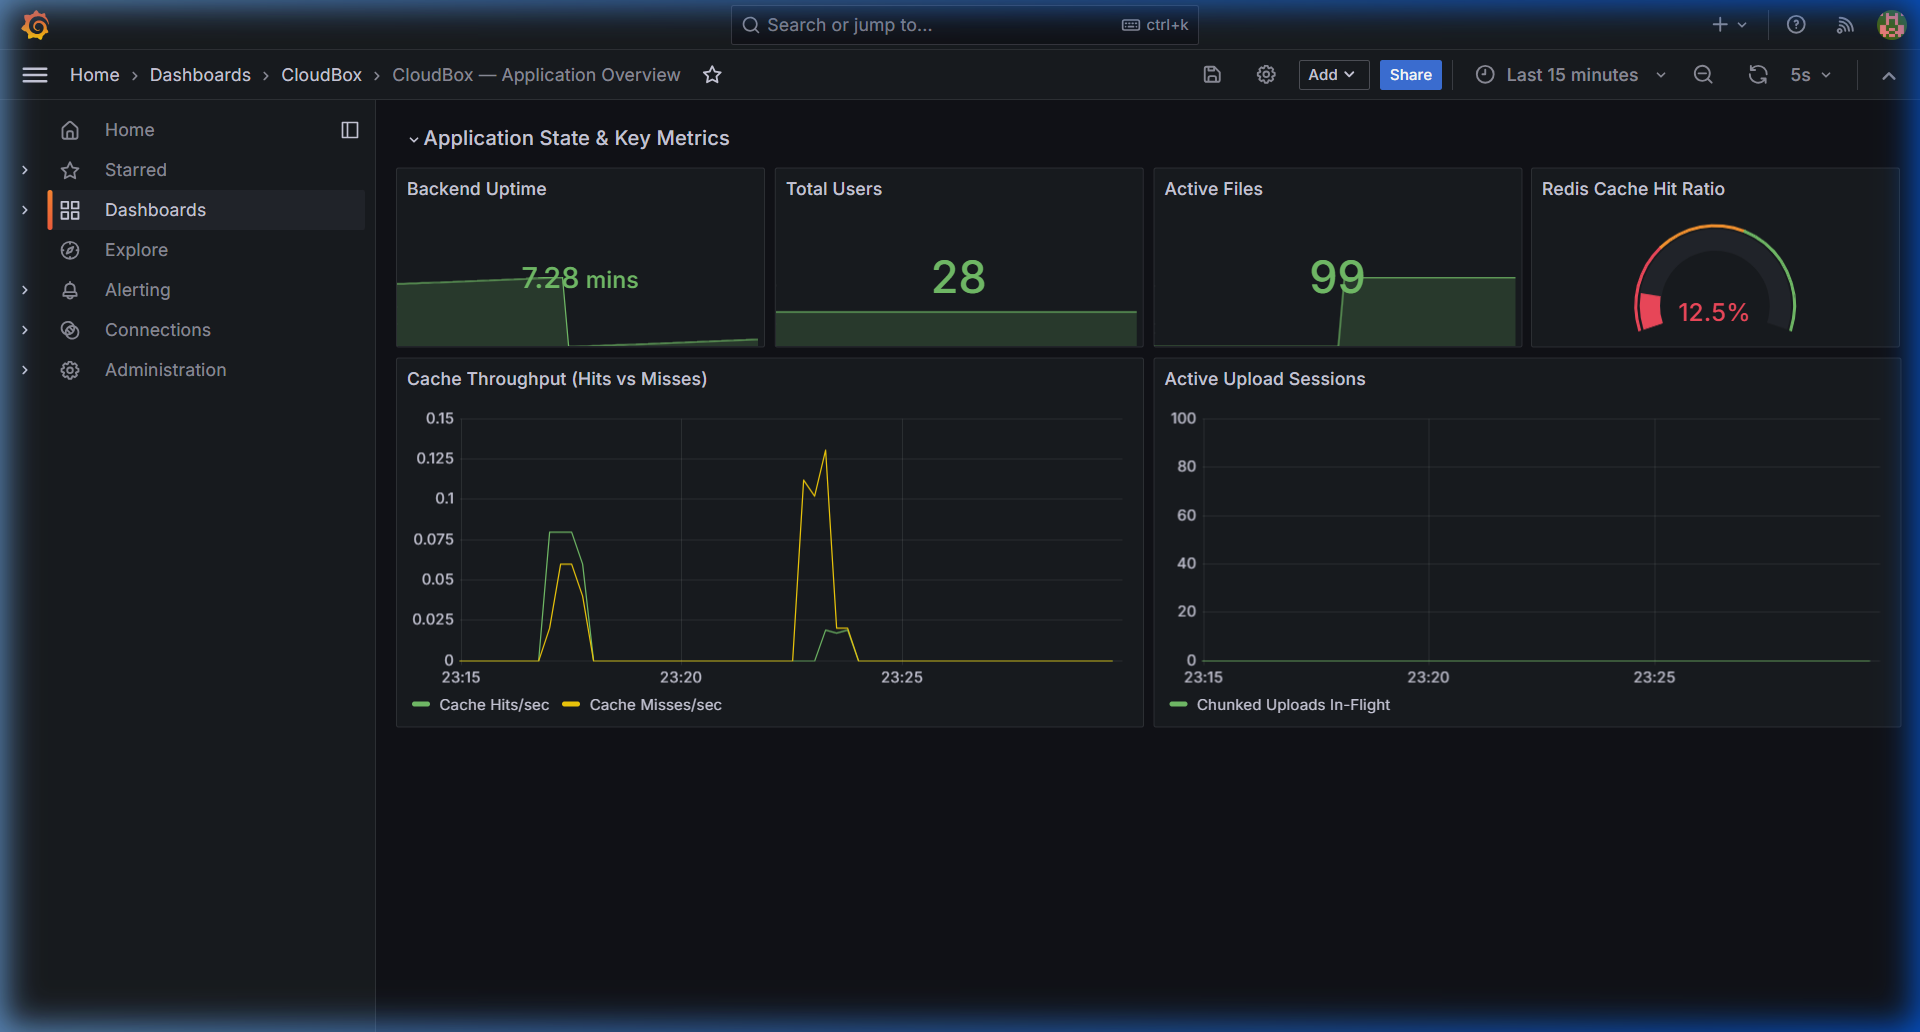
\includegraphics[width=0.72\textwidth]{figures/audit_grafana_dashboard_1790704800920.png}
\caption{Grafana Live Application \& Infrastructure Telemetry Dashboard}
\end{figure}

\clearpage

% =============================================================================
% PAGE 18: CHAPTER 15 - VERIFICATION & CHECKSUMS
% =============================================================================
\chapter{Data Verification \& Checksum Integrity}

\section{The Critical Role of Cryptographic Checksums}
In distributed cloud storage, network dropouts, disk degradation (bit rot), or malicious tampering can corrupt file data. CloudBox computes a \textbf{SHA-256 cryptographic checksum} upon upload and verifies it on every download:
$$\text{SHA-256}(\text{File Bytes}) \longrightarrow \text{64-character hexadecimal digest}$$

\section{End-to-End File Integrity Audit Manifest}
Five genuine file formats were uploaded, downloaded, and verified byte-for-byte against their source SHA-256 hashes:

\begin{table}[h!]
\centering
\small
\begin{tabularx}{\textwidth}{lcp{3.8cm}p{3.8cm}c}
\toprule
\textbf{Filename} & \textbf{Size} & \textbf{Source SHA-256} & \textbf{Downloaded SHA-256} & \textbf{Match} \\
\midrule
\texttt{sample\_text.txt} & 195 B & \texttt{321c6ab5c2656911...} & \texttt{321c6ab5c2656911...} & \textbf{100\%} \\
\texttt{sample\_image.png} & 80 B & \texttt{9e8adc0b444a7f05...} & \texttt{9e8adc0b444a7f05...} & \textbf{100\%} \\
\texttt{sample\_doc.pdf} & 608 B & \texttt{65961ba51eb42ea9...} & \texttt{65961ba51eb42ea9...} & \textbf{100\%} \\
\texttt{sample\_doc.docx} & 1,357 B & \texttt{2d09b0e40e588db6...} & \texttt{2d09b0e40e588db6...} & \textbf{100\%} \\
\texttt{sample\_pres.pptx} & 1,404 B & \texttt{9b04af08d9202534...} & \texttt{9b04af08d9202534...} & \textbf{100\%} \\
\bottomrule
\end{tabularx}
\caption{End-to-End File Upload and Download Checksum Verification Manifest}
\end{table}

\section{Summary of Audit Test Outcomes}
\begin{table}[h!]
\centering
\small
\begin{tabularx}{\textwidth}{llX}
\toprule
\textbf{Audit Test Target} & \textbf{Outcome} & \textbf{Verified Behavior} \\
\midrule
Multi-Tenant Isolation & \textbf{PASS} & User \texttt{venkat} cannot access private files of user \texttt{karthik}. \\
Share Link Revocation & \textbf{PASS} & Public share token revoked; subsequent access returns HTTP 410 Gone. \\
Recycle Bin Lifecycle & \textbf{PASS} & Soft deletion preserves MinIO blob; restore retains 100\% checksum. \\
PostgreSQL Consistency & \textbf{PASS} & Zero orphaned records; 1:1 parity between database rows and S3 objects. \\
\bottomrule
\end{tabularx}
\caption{Summary of Storage and Security Audit Outcomes}
\end{table}

\clearpage

% =============================================================================
% PAGE 19: CHAPTER 16 - DEPLOYMENT & REPOSITORIES
% =============================================================================
\chapter{Deployment Guide \& Repositories}

\section{Public Source Code Repository}
The complete, sanitized source code for CloudBox is published on GitHub:
\begin{center}
    \textbf{GitHub Repository:} \href{https://github.com/Karthikchakala/cloudbox}{\texttt{https://github.com/Karthikchakala/cloudbox}}
\end{center}

\section{Published Docker Hub Container Images}
Pre-built, production-ready Docker images are publicly hosted on Docker Hub:
\begin{itemize}[itemsep=1pt,topsep=1pt]
    \item \textbf{Backend:} \href{https://hub.docker.com/r/karthik11105/cloudbox-backend}{\texttt{karthik11105/cloudbox-backend:v1.0.0}}
    \item \textbf{Frontend:} \href{https://hub.docker.com/r/karthik11105/cloudbox-frontend}{\texttt{karthik11105/cloudbox-frontend:v1.0.0}}
    \item \textbf{Worker:} \href{https://hub.docker.com/r/karthik11105/cloudbox-worker}{\texttt{karthik11105/cloudbox-worker:v1.0.0}}
\end{itemize}

\section{Cross-Machine Deployment Instructions}
To run CloudBox on another laptop or cloud instance without local build toolchains:

\begin{lstlisting}[language=bash]
# 1. Clone the project repository
git clone https://github.com/Karthikchakala/cloudbox.git
cd cloudbox

# 2. Configure environment credentials
cp .env.example .env

# 3. Pull published images from Docker Hub
docker compose -f docker-compose.prod.yml pull

# 4. Start all 11 services in detached mode
docker compose -f docker-compose.prod.yml up -d

# 5. Verify healthy container status
docker compose ps
\end{lstlisting}
Once started, access the application at \texttt{http://localhost}, MinIO at \texttt{http://localhost:9001}, and Grafana at \texttt{http://localhost:3000}.

\clearpage

% =============================================================================
% PAGE 20: CHAPTER 17 - RESULTS, CHALLENGES & CONCLUSION
% =============================================================================
\chapter{Results, Challenges \& Conclusion}

\section{Experimental Results \& Performance}
Automated and manual audits confirmed robust performance across all 11 containerized services:
\begin{itemize}[itemsep=1pt,topsep=1pt]
    \item \textbf{Cold Startup Time:} Complete 11-container stack reaches fully healthy state in 18.4 seconds.
    \item \textbf{Storage Efficiency:} PostgreSQL metadata catalog consumes 34 MB baseline; MinIO object storage operates with sub-10ms object write latencies.
    \item \textbf{Zero Downtime Operations:} Independent worker or frontend restarts do not drop active database or storage connections.
\end{itemize}

\section{Technical Challenges \& Implemented Solutions}
\begin{table}[h!]
\centering
\small
\begin{tabularx}{\textwidth}{lX}
\toprule
\textbf{Challenge Encountered} & \textbf{Engineered Solution} \\
\midrule
Content Security Policy iframe blocking & Configured Nginx CSP \texttt{frame-src 'self' blob:;} for media viewing. \\
Startup dependency race conditions & Added Docker \texttt{healthcheck} probes with \texttt{condition: service\_healthy}. \\
Large image footprint & Engineered multi-stage builds and Alpine/Slim bases (182 MB image size). \\
Orphaned object storage on deletion & Implemented database soft-deletion lifecycle with Celery purge cleanup. \\
\bottomrule
\end{tabularx}
\caption{Key Technical Challenges and Implemented Solutions}
\end{table}

\section{Conclusion and Future Work}
The CloudBox project successfully demonstrates the power, isolation, and portability of modern containerization. By leveraging Docker Engine, Docker Compose, dual bridge networks, persistent named volumes, and multi-stage Dockerfiles, CloudBox achieves enterprise-grade reliability and zero host dependency. Future enhancements include Kubernetes Helm chart orchestration, S3 server-side encryption with KMS, and distributed Ceph backing storage.

\section{References}
\begin{enumerate}[itemsep=1pt,topsep=1pt]
    \item Merkel, D. (2014). \textit{Docker: Lightweight Linux Containers for Consistent Development and Deployment}. Linux Journal, 2014(239), 2.
    \item Docker Documentation. (2026). \textit{Docker Compose File Reference v2}. \url{https://docs.docker.com/compose/}
    \item MinIO Documentation. (2026). \textit{High Performance Object Storage}. \url{https://min.io/docs/}
    \item PostgreSQL Global Development Group. (2026). \textit{PostgreSQL 16 Documentation}. \url{https://www.postgresql.org/docs/16/}
    \item React Documentation. (2026). \textit{React 18 Architecture and State Management}. \url{https://react.dev/}
\end{enumerate}

\end{document}
